\chapter{Communication}

\paragraph*{}
This chapter details the exploratory results for the sub-task \textbf{Communication in the Swarm}. This task has been tackled under the assumption that the \textit{swarm fleet are capable of object detection}, which is a necessary premise to parallelize the workload as another group member is working on it. Some other vital constraints include:

\begin{itemize}
    \item \textbf{Robots are stationary} \\
    This is assumed because we can temporarily exclude motor control for simplicity
    \item \textbf{Robots are on fixed coordinates configured by the user} \\
    This is assumed because robots can communicate their coordinates to other fleet members and the assumption offers an easy method to check for the correctness in their communication.
    \item \textbf{Start with 5 robots during simulation} \\
    This constraint is to minimize the complexity in the environment
\end{itemize}

\paragraph*{}
After thorough consideration and evaluation, the best simulating environment for this specific communication task is Webots from Cyberbotics. Webots provide the PROTO mechanism for developers to build and reuse complex objects. This allows us to simulate and test our assumptions upon pre-built objects, such as 
TurtleBot. 

\begin{figure}[H]
    \centering
    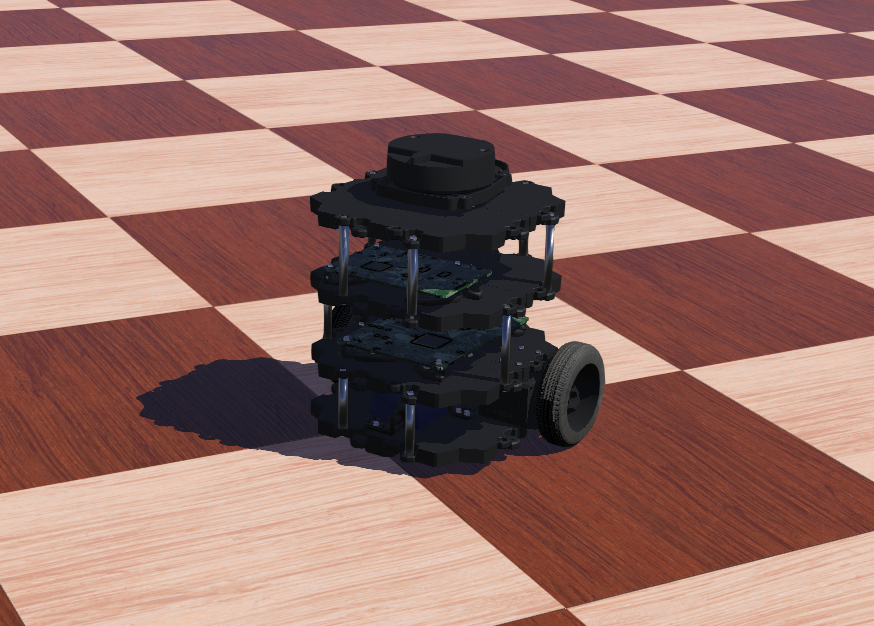
\includegraphics[width=0.4\linewidth]{assets/images/communication/environment/turtlebot.png}
    \caption{TurtleBot 3 Burger in Webots}
    \label{fig:turtlebot}
\end{figure}

In webots, the version of the TurtleBot given in the PROTO nodes is the Burger model of the third version of the TurtleBot robot Figure \ref{fig:turtlebot}.  Moreover, the TurtleBot has two functioning motors and a 360-degree distance sensor, allowing it to do simple navigation. However, using TurtleBot alone is inadequate to simulate the communication framework. Therefore, three more basic nodes are added to the TurtleBot object, which are the following: Firstly, the GPS node (Figure \ref{fig:GPS}), this module is installed to obtain the robot's position in the simulated world. This direct approach is used because the localization and mapping process is not accounted for in this testing. Secondly, the Emitter node (Figure \ref{fig:Emitter}), this module is added to the robot to model a broadcast behavior. Additionally, Webots allows the developer to configure the properties of the Emitter Class; for instance, the emission range. Thirdly, the Receiver node (Figure \ref{fig:Receiver}), this module is connected as an accompaniment to the Emitter Class, because the Emitter node does not support both emitting and receiving functionalities. The receiver listens for incoming data packets and appends them to the tail of a queue. Moreover, incoming data packets will be discarded if the receiver's buffer size is exceeded. By combining all the devices, an abstract simulation of swarm robotics communication approaches can now be validated.

\begin{figure}[!htb]
    \minipage{0.32\textwidth}
        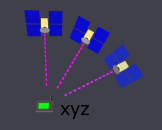
\includegraphics[width=\linewidth]{assets/images/communication/devices/gps.png}
        \caption{GPS node}\label{fig:GPS}
    \endminipage\hfill
    \minipage{0.32\textwidth}
        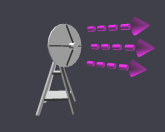
\includegraphics[width=\linewidth]{assets/images/communication/devices/emitter.png}
        \caption{Emitter node}\label{fig:Emitter}
    \endminipage\hfill
    \minipage{0.32\textwidth}%
        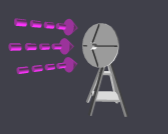
\includegraphics[width=\linewidth]{assets/images/communication/devices/receiver.png}
        \caption{Receiver node}\label{fig:Receiver}
    \endminipage
\end{figure}

\paragraph*{}
The main approach to communication in the swarm would be to gain awareness over robotic members in the swarm system and finding consensus within the swarm before any further follow-up actions are taken. In case of an object getting detected, the first robot that detects the object would act as the task master, supplying other robots in the swarm with the object's coordinates. Consensus is essential for this use case because every swarm members have to agree on the object detection before any actions. Therefore, we are utilizing modes to build a central template code to operate the swarm. There are two main modes for the swarm: \textbf{Idle} mode and \textbf{Consensus} mode.

\paragraph*{}
The \textbf{Idle} mode entails the period where fleet members are setting themselves up by communicating their \textbf{identifiers} and their \textbf{coordinates}, which the receivers store as internal dictionaries. Figure \ref{fig:idle_mode} displays the functional instance where the turtlebots in the environment are aware of other members and their respective coordinates and test-print them on console.

\begin{figure}[H]
    \centering
    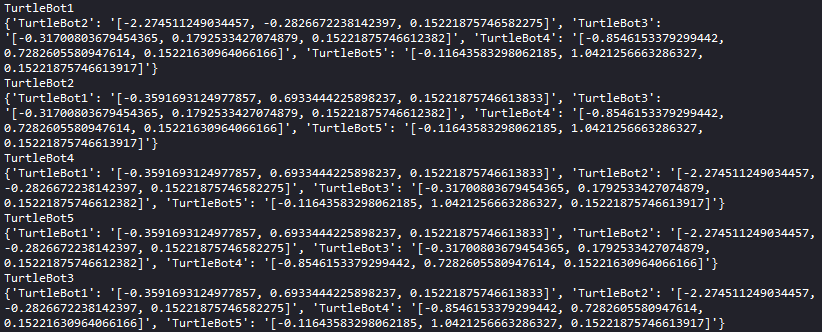
\includegraphics[width=1\linewidth]{assets/images/communication/outputs/idle_mode.png}
    \caption{Idle Mode}
    \label{fig:idle_mode}
\end{figure}

\paragraph*{}
The \textbf{Consensus} mode occurs when an object is "detected" by any of the swarm members. After the detection, the robot which identifies the object will switch its mode to Consensus and save the object's coordinates. Consequently, it will communicate to other members of the present object, readying them for any subsequent actions. In this test case, a set of object coordinates is manually supplied to one of the members after four seconds. Figure \ref{fig:consensus_mode} shows \textit{TurtleBot2}, a member in the environment, receiving the set of coordinates and communicating to the swarm that it is the task master and the location of the object, thereby bumping other robots' modes to Consensus mode.

\begin{figure}[H]
    \centering
    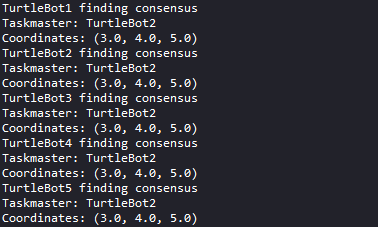
\includegraphics[width=0.6\linewidth]{assets/images/communication/outputs/consensus_mode.png}
    \caption{Consensus Mode}
    \label{fig:consensus_mode}
\end{figure}

\paragraph*{}
This approach can be improved by planning for worst-case-scenarios in advance. To expand further, this can be from preventing any race conditions occurring from the consensus mode, and including an extra verification step after communication. However, a potential challenge with the verification step is that robotic communication is extensive; having additional communication demands should be in balance with the available resources the robots allow.

\paragraph*{}
Additionally, the \textbf{application layer} is currently sending and receiving:

\begin{itemize}
    \item Robot's identifier
    \item Robot's coordinates
    \item Object coordinates
\end{itemize}

We will potentially require more information to be transmitted with additional requirements from other modules, which is another area for further improvements.
